\documentclass[main]{subfiles} 

\begin{document}

\chapter{ALGORITHM DEVELOPMENT AND FLOWCHART}

\section{Algorithm}
	\subsection{Algorithm for State Machine}
	
\begin{minted}[breaklines]{text}
if isAdding ==true:
    if stack is not empty and isReplacing == true:
        pop the top state at stack
    else if stack is not empty:
        pause the top state at stack

     push new state to stack
     init top of the stack

     isAdding = false


if isRemoving==true and stack is not empty:
    pop the top state of stack
    
    if stack is not empty:
        resume the top state at stack

    isRemoving = false
\end{minted}


	\subsection{Algorithm for Splash Screen State}

\begin{minted}{text}
load sprites
x = 0
loop{
    x++
    display sprite no x
    if x == 12 go to main menu
}


	\end{minted}
	
	\subsection{Algorithm for Main Menu State}
        \begin{minted}{text}
load sprites
display the sprites
play theme music
loop{
    if play button is clicked or enter is pressed{
        stop theme music
        player1 score = player 2 score = 0
        time = 0 
        go to game state
    }
    if about button is clicked:
        go to about screen 
    if instructions button is clicked:
        go to instructions screen
    if exit button is clicked:
        exit the game
}

    \end{minted}	

	\subsection{Algorithm for Game State}
	\begin{minted}[breaklines]{text}
load the sprites
set the position of players and ball
display the sprites for the environment and players
resume time
isSecondHalf = false
loop{
    get input from players for movement

    if player moves left or right:
        animate the player
        change its position

    if player jumps:
        apply linear velocity  upwards
    if player presses kick button {
        check if ball collides the player
        if player collides the ball {
            play kick sfx
            apply force to the ball at the direction respective to its relative position with the player
        }
    }
    
    display the score and time

    process the world in Box2D by one step
    process the position of players and ball

    if position of ball lies in the bounds of goal post:
        play goal sfx
        score of respective player += 1
        reposition the player and ball

    if game time >= 45 and isSecondHalf == false:
        pause time
        isSecondHalf = true
        go to half time state

    if game time >= 90:
        go to game over state
        
    display the ball and players at its respective position
}
	\end{minted}

\pagebreak

	\subsection{Algorithm for Game Over State}
\begin{minted}{text}

load sprites 
display the sprites

if player 1 score > player 2 score:
    display "Player 1 Wins"
else if player 2 score > player 1 score:
    display "Player 2 Wins"
else:
    display "Match Tied"

loop{
    if replay button is clicked:
        restart timer
        player 1 score = player 2 score = 0
        go to game state

    if exit button is clicked:
        exit the game
}

\end{minted}
	
	
	
\newpage
\section{Flowchart}
    \subsection{Flowchart for State Machine State}
        \begin{figure}[H]
            \centering
            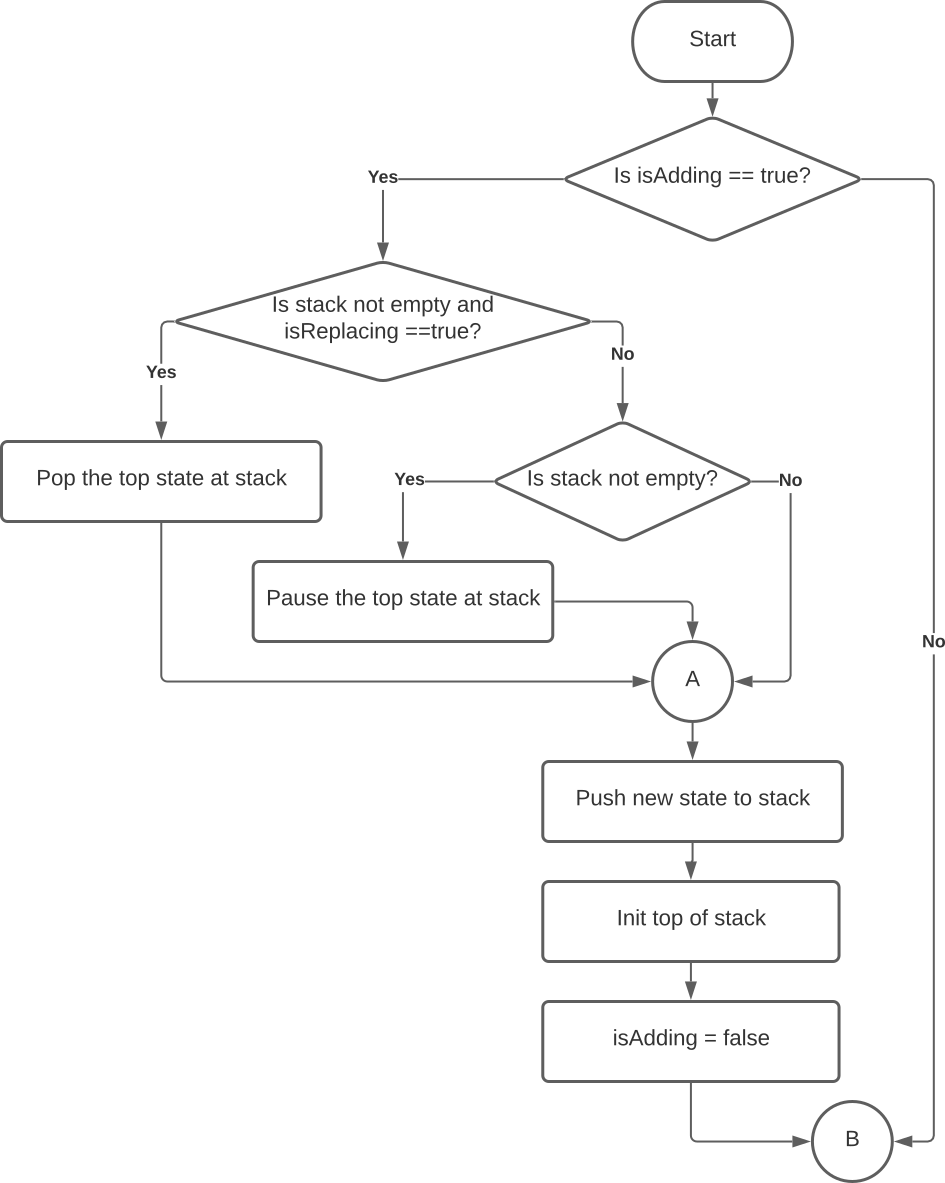
\includegraphics[scale=0.5]{graphics/flowcharts/state_machine1.png}
            \caption{Flowchart for State Machine A}
            \label{fig:state_machineA}
        \end{figure}
        
        \begin{figure}[H]
            \centering
            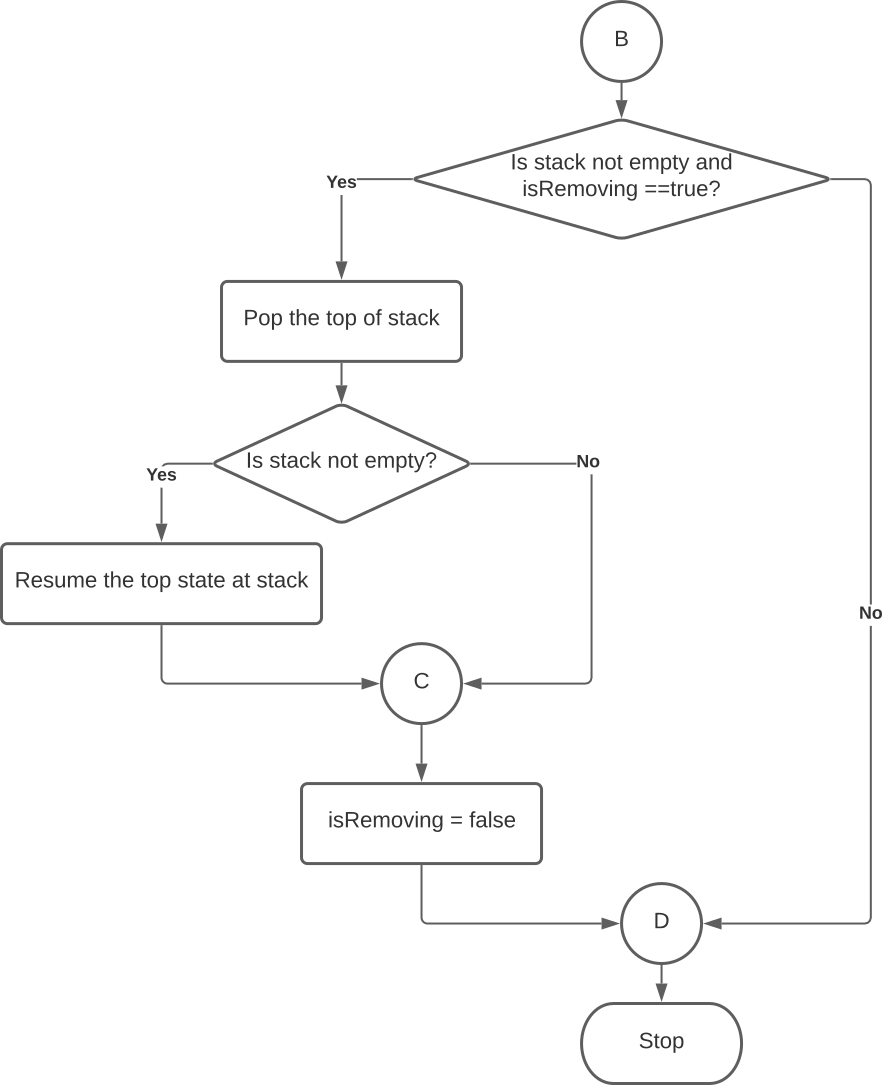
\includegraphics[scale=0.5]{graphics/flowcharts/state_machine2.png}
            \caption{Flowchart for State Machine B}
            \label{fig:state_machineB}
        \end{figure}
        


	\subsection{Flowchart for Splash Screen}

        \begin{figure}[H]
            \centering
            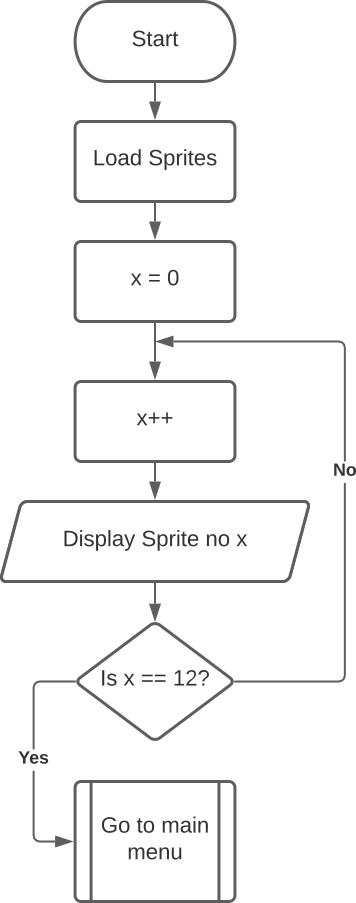
\includegraphics[scale=0.5]{graphics/flowcharts/splash_screen.png}
            \caption{Flowchart for Splash Screen State}
            \label{fig:splash_screen}
        \end{figure}

	\subsection{Flowchart for Main Menu State}
	    \begin{figure}[H]
	        \centering
	        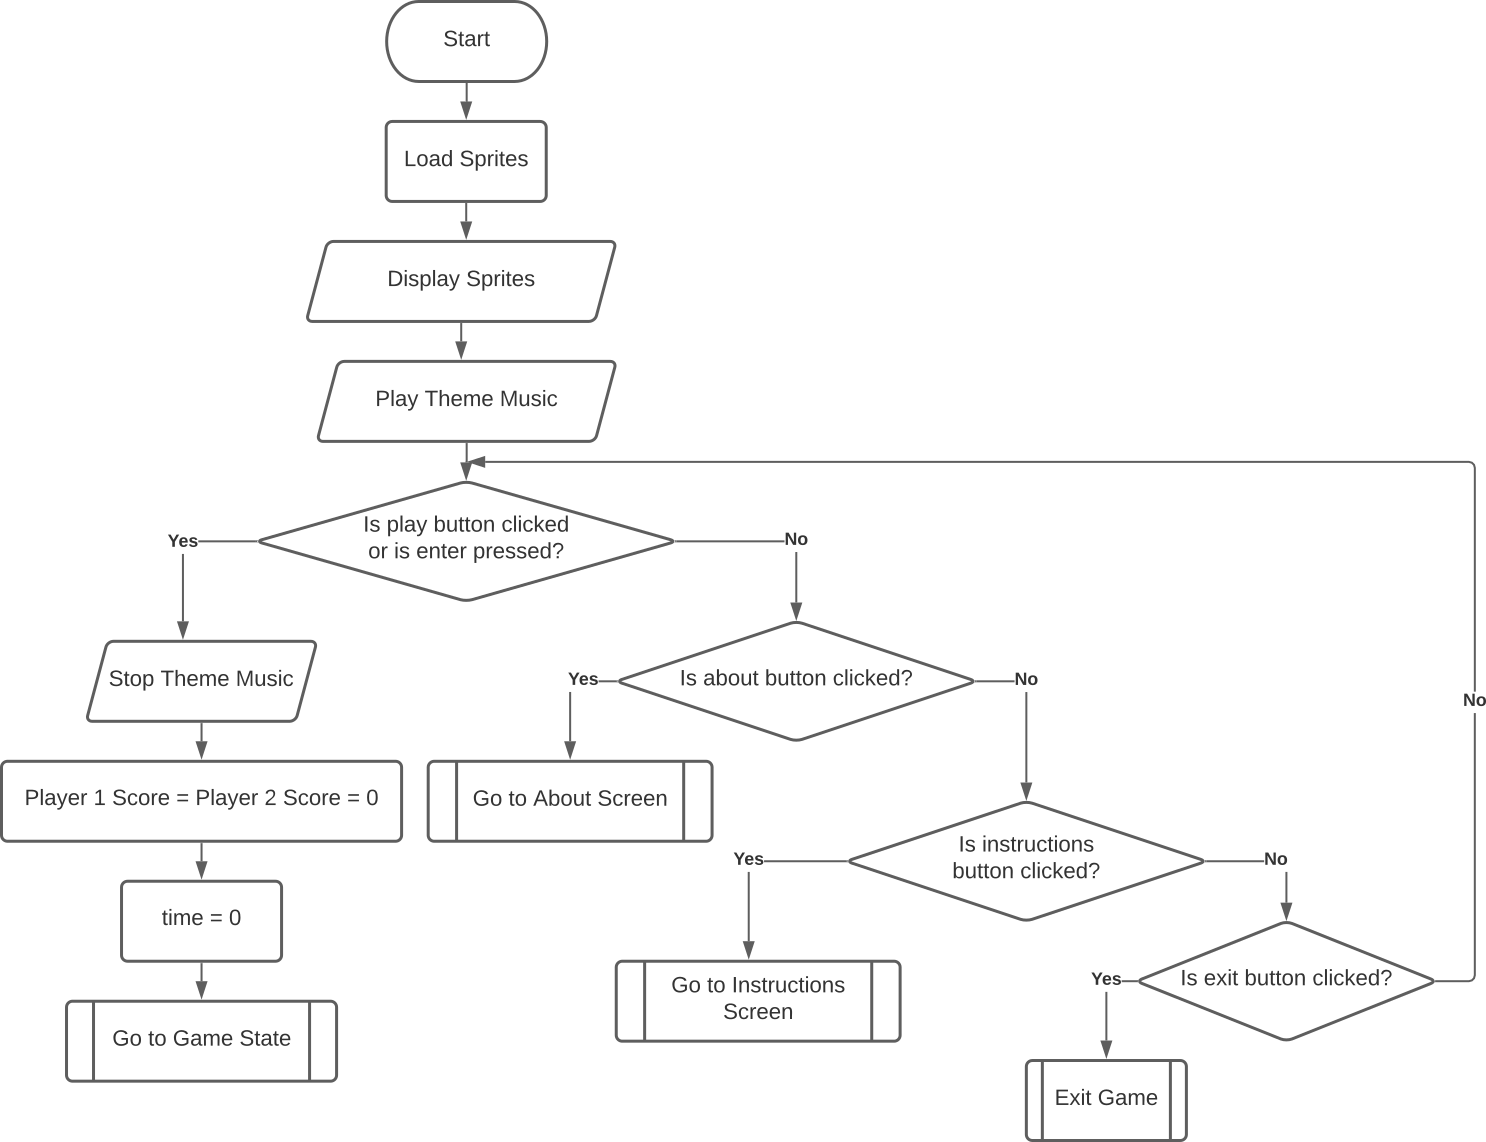
\includegraphics[scale=0.4]{graphics/flowcharts/main_menu.png}
	        \caption{Flowchart for Main Menu State}
	        \label{fig:main_menu}
	    \end{figure}
	
	
	\subsection{Flowchart for Game State}
        \begin{figure}[H]
            \centering
            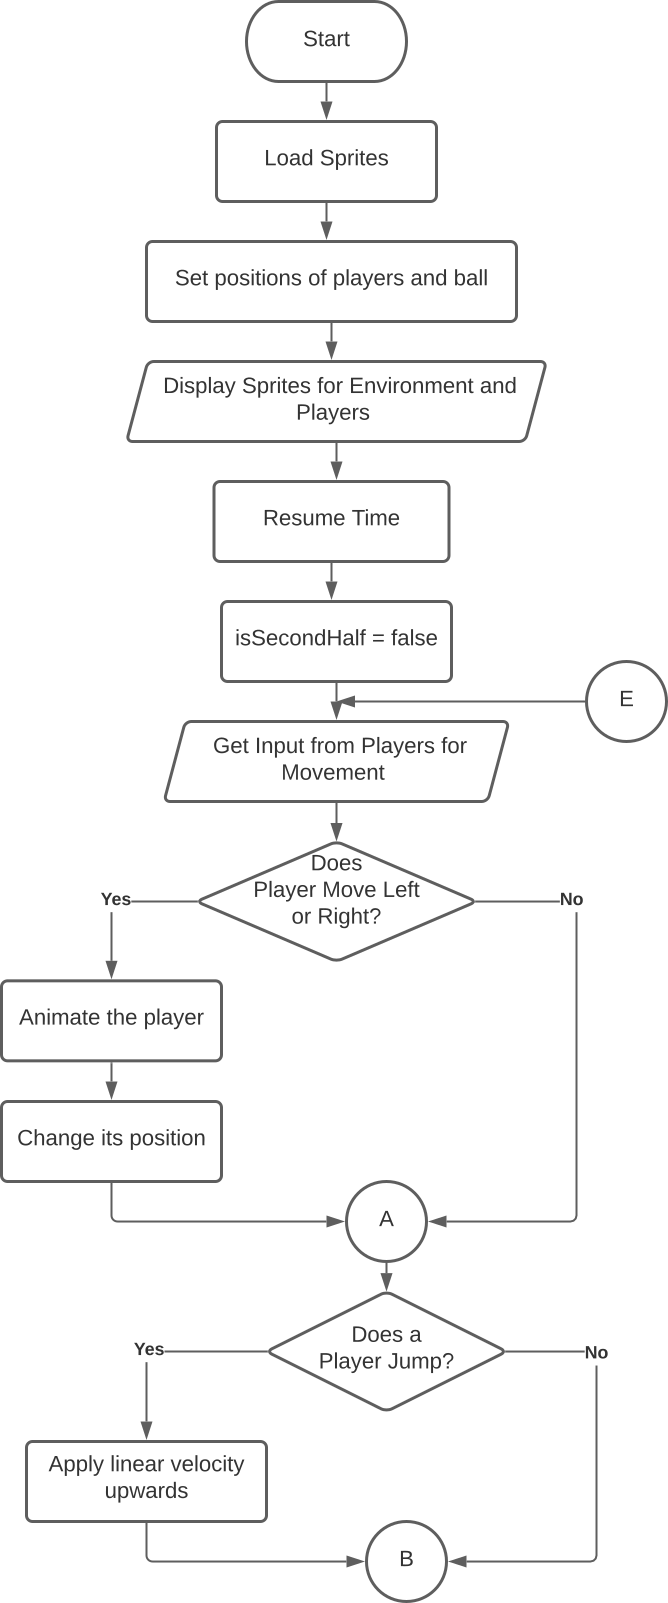
\includegraphics[scale=0.5]{graphics/flowcharts/game_state1.png}
            \caption{Flowchart for Game State A}
            \label{fig:gamestateA}
        \end{figure}	
        
        \begin{figure}[H]
            \centering
            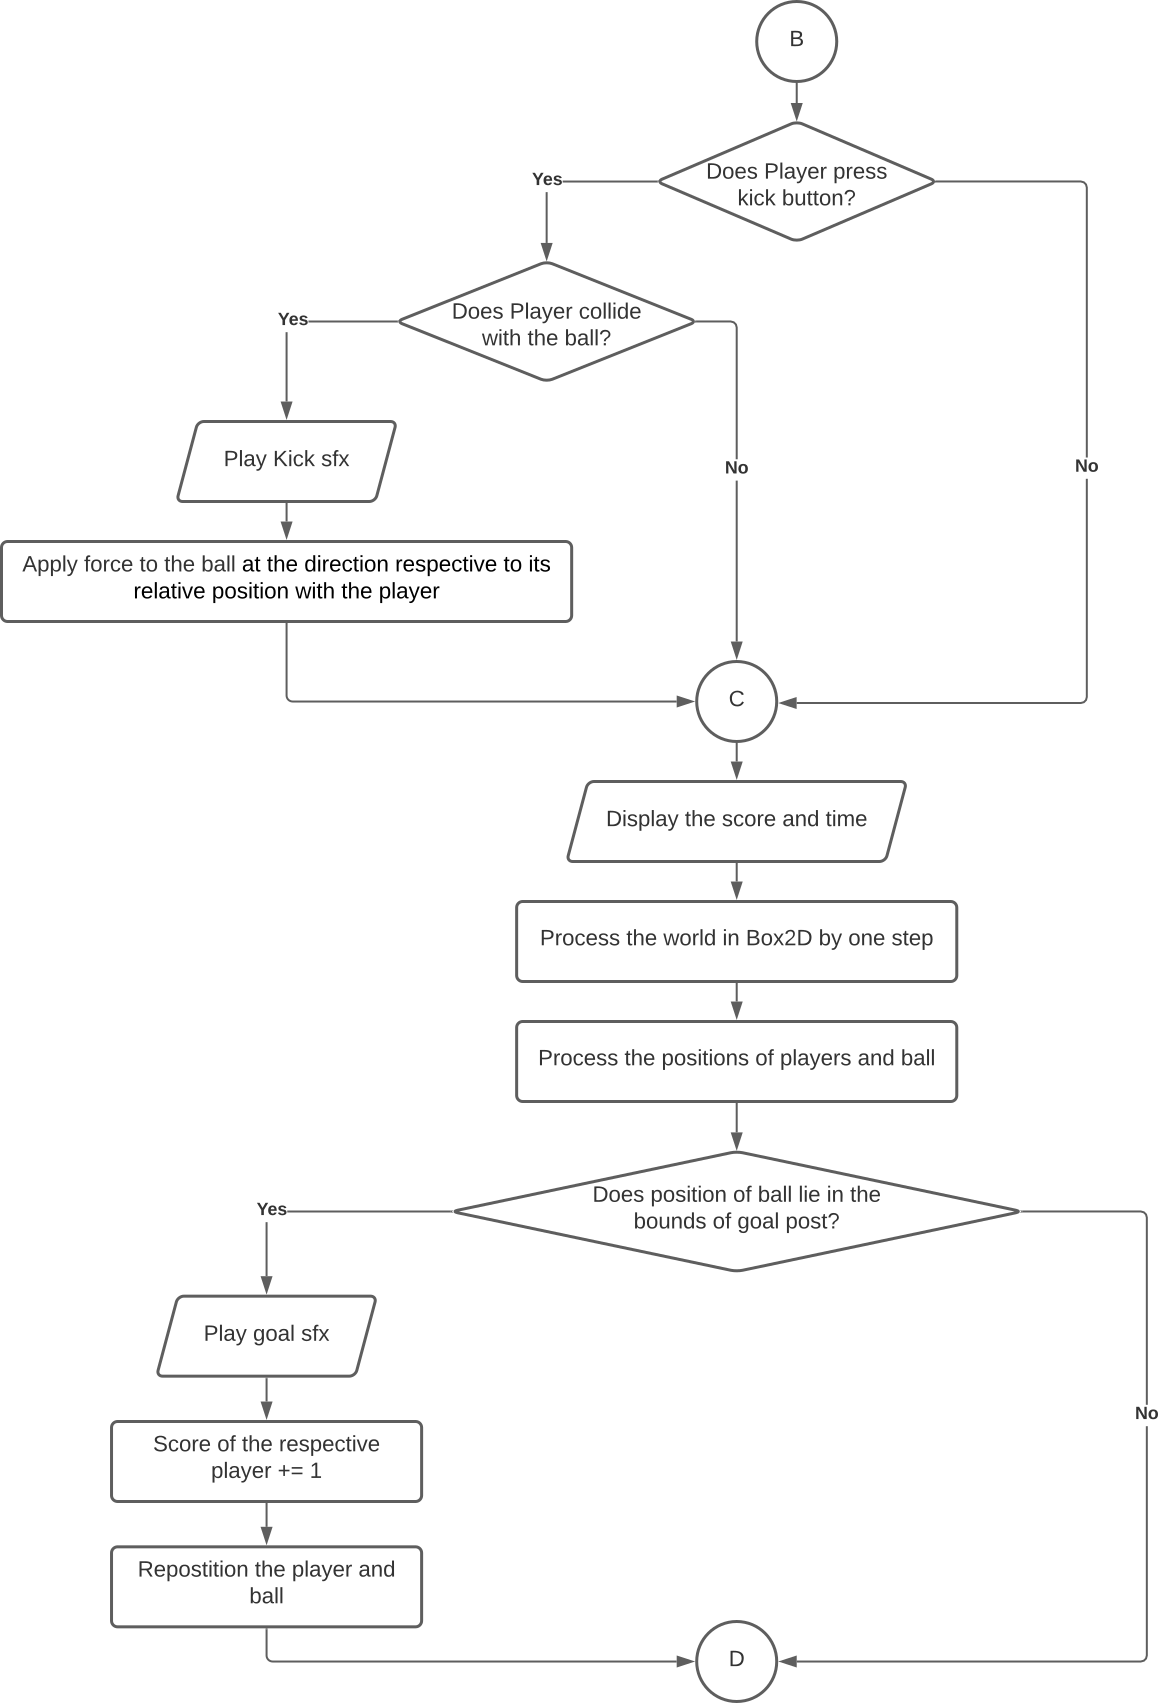
\includegraphics[scale=0.5]{graphics/flowcharts/game_state2.png}
            \caption{Flowchart for Game State B}
            \label{fig:gamestateB}
        \end{figure}
        
        \begin{figure}[H]
            \centering
            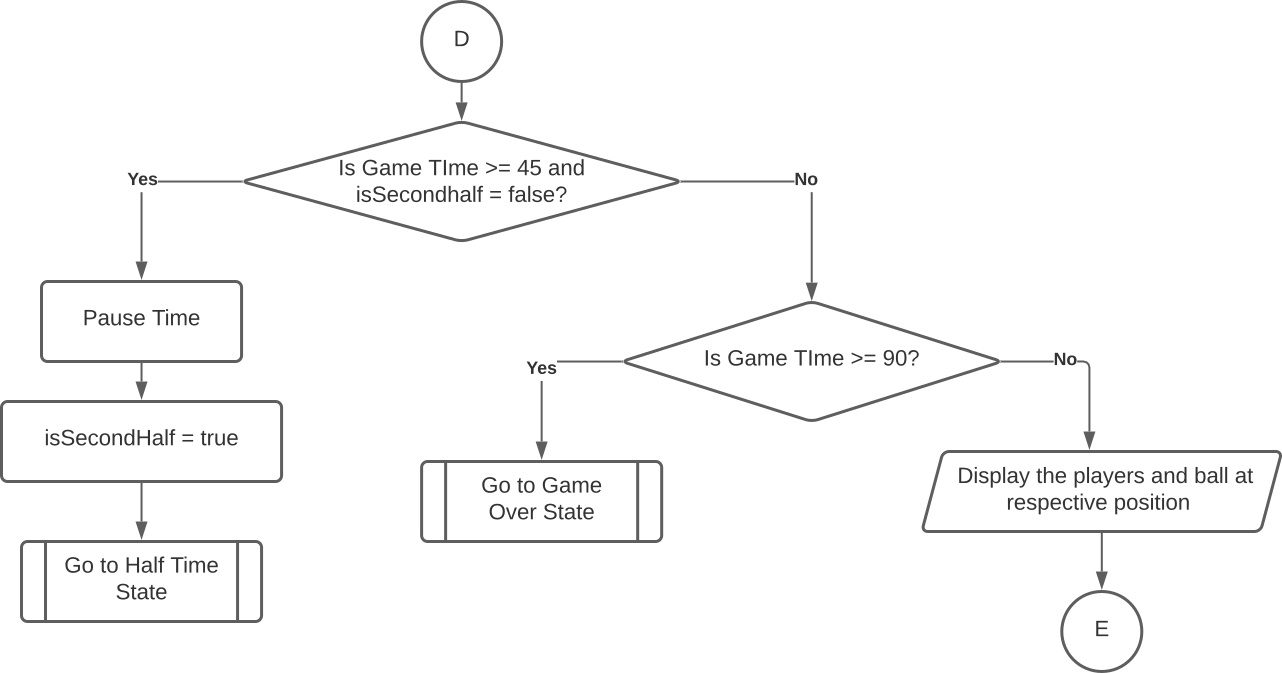
\includegraphics[scale=0.5]{graphics/flowcharts/game_state3.png}
            \caption{Flowchart for Game State C}
            \label{fig:gamestateC}
        \end{figure}	
        
    \subsection{Flowchart for Game Over State}
        \begin{figure}[H]
            \centering
            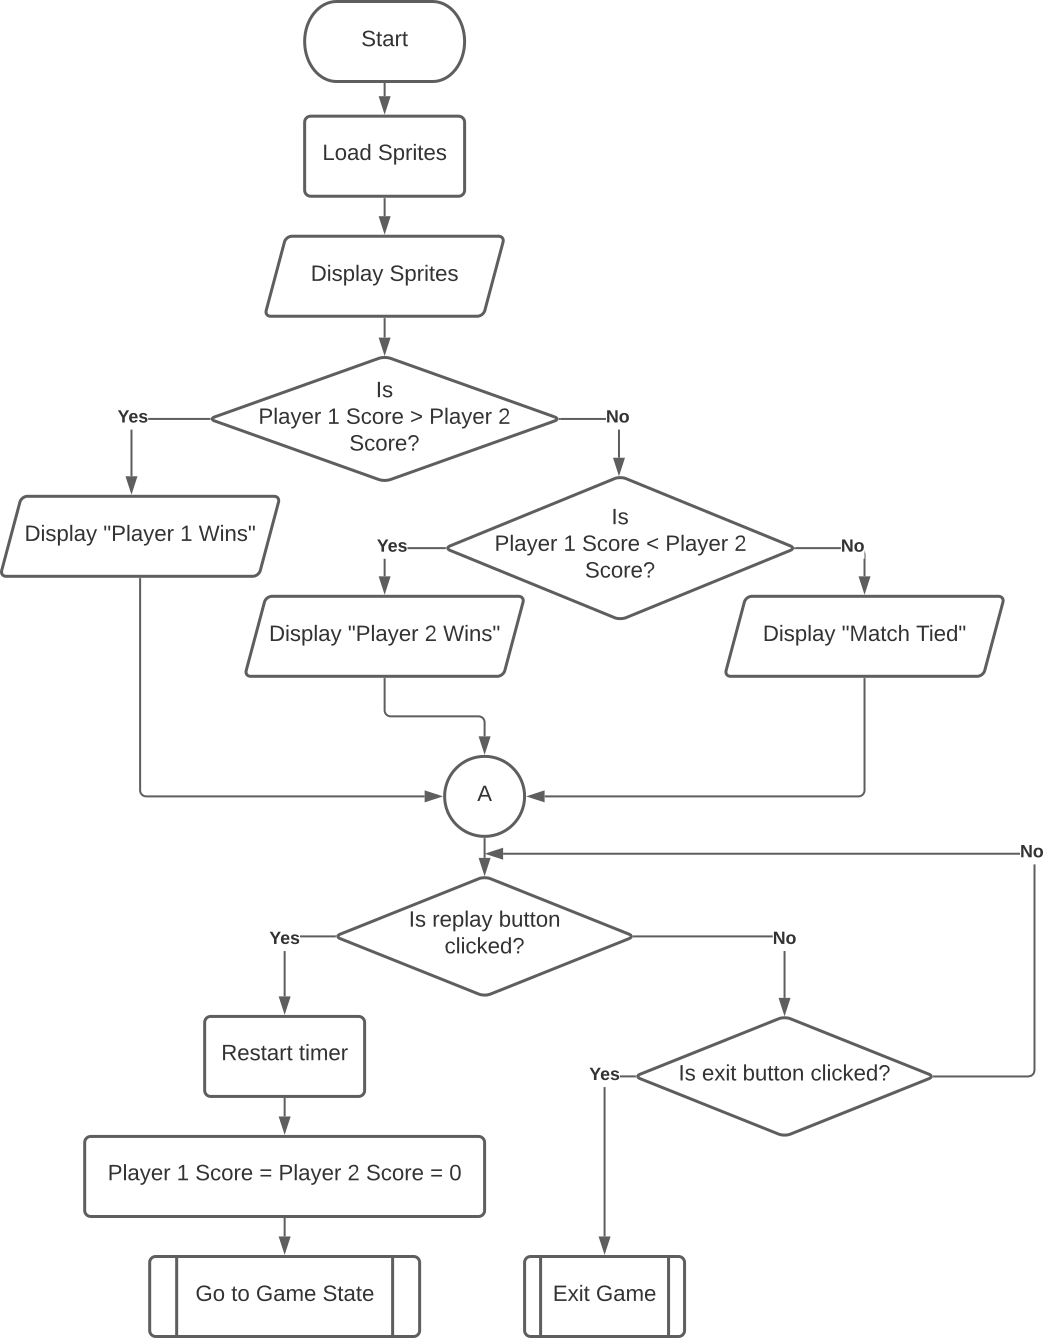
\includegraphics[scale=0.5]{graphics/flowcharts/gameover_state.png}
            \caption{Flowchart of Game Over State}
            \label{fig:GameOverState}
        \end{figure}



\section{UML Diagrams}
    \subsection{Collaboration diagram for GameState class}

\begin{figure}[H]
    \centering
    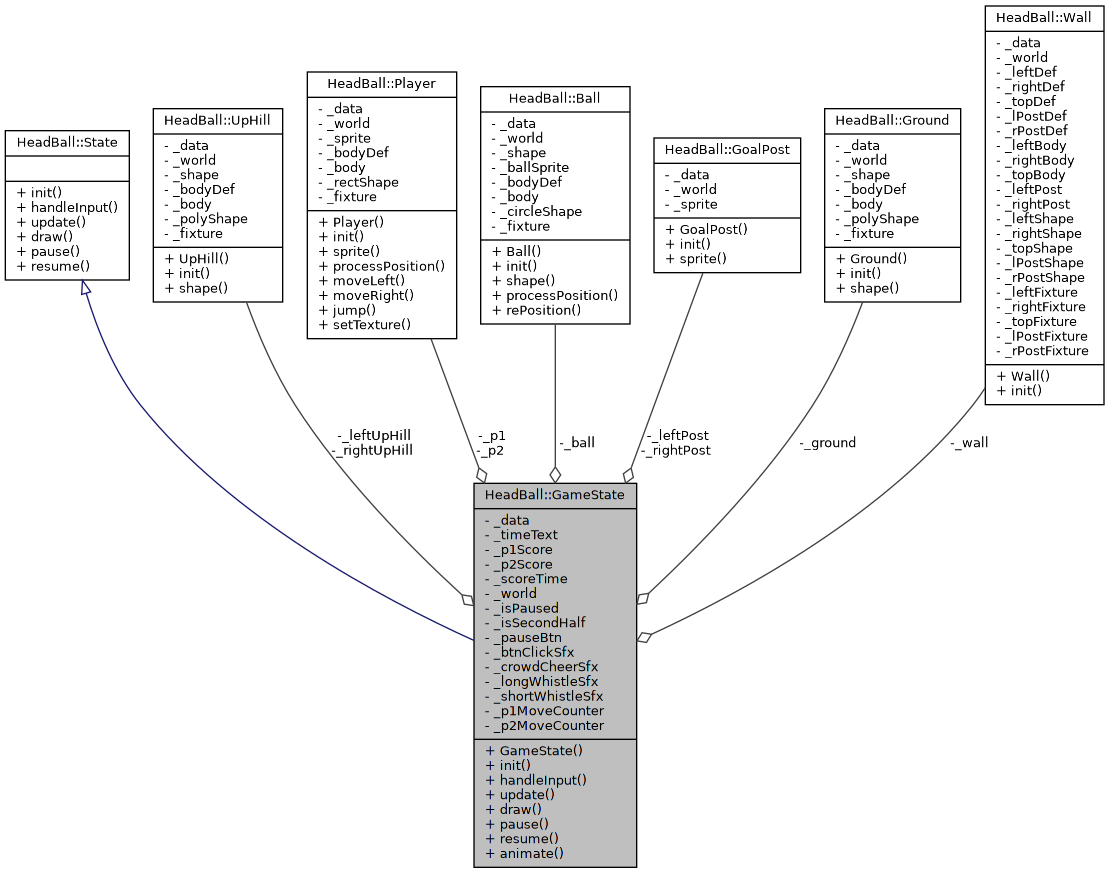
\includegraphics[scale=0.4]{graphics/UML_diagrams/gamestate_collab.png}
    \caption{Collaboration diagram for GameState class}
    \label{fig:collaboration_diagram_GameState}
\end{figure}

\newpage

\subsection{State Class Hierarchy Diagram}
\begin{figure}[H]
    \centering
    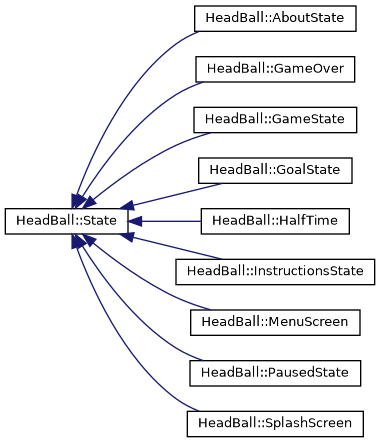
\includegraphics[scale=0.5]{graphics/UML_diagrams/state_hierarchy_brief.png}
    \caption{State Class Hierarchy Diagram}
    \label{fig:state_hierarchy_brief}
\end{figure}

\subsection{Inheritance diagram for State Class}
\begin{figure}[H]
    \centering
    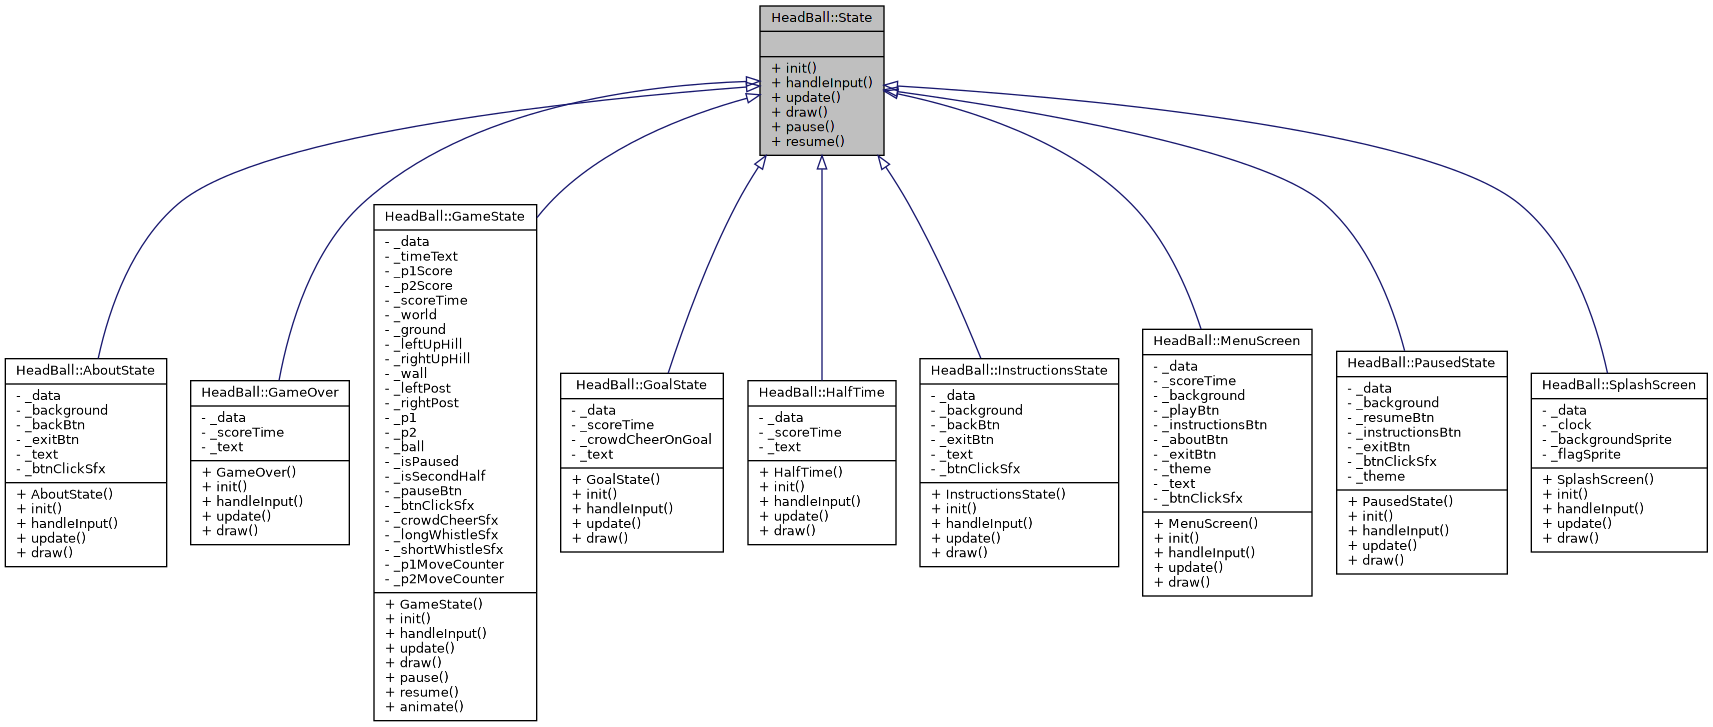
\includegraphics[scale=0.275]{graphics/UML_diagrams/state_hierarchy_full.png}
    \caption{Inheritance diagram for State Class}
    \label{fig:state_hierarchy_full}
\end{figure}

\end{document}
